\documentclass[a4paper]{article}
\linespread{1.6}
\usepackage{enumerate}
\usepackage{geometry}
\usepackage{setspace}
\usepackage{amsmath}
\usepackage{amssymb}
\usepackage{cite}
\usepackage[pdftex]{graphicx}
\usepackage{float}
\usepackage{subfigure}
\usepackage{listings}
\geometry{left=1.4cm,right=1.4cm,top=2.5cm,bottom=2.5cm}

\begin{document}
\begin{spacing}{2.0}
\begin{flushleft}\begin{huge}EEL5840 Fundamental Machine Learning   Homework 6\end{huge}\end{flushleft}
\begin{flushright}\begin{Large} Hudanyun Sheng \end{Large}\end{flushright}

\Large{All the code used in this report are attached at the end of this report.}
\normalsize
\begin{itemize}

\item An illustration of my network's architecture is shown:
\begin{figure}[H]
\centering
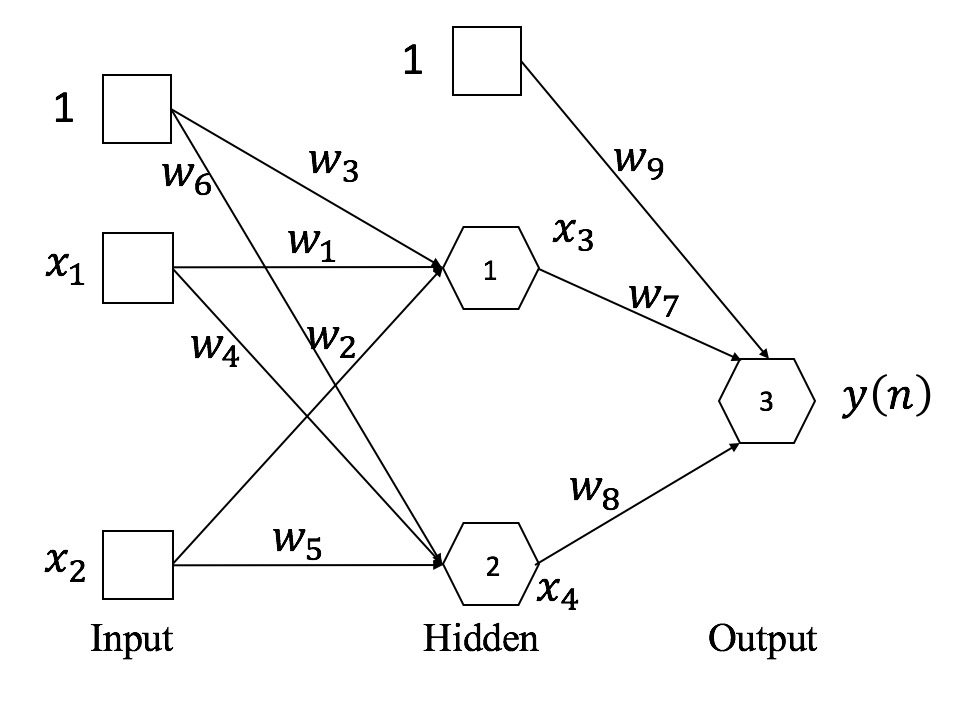
\includegraphics[width = 5in]{flowchart.png}
\caption{Illustration of the multiple-layer perceptron neural network}
\label{flowchart}
\end{figure}
There is only one hidden layer in the network I defined. There are 2 processing units in the input layer, 2 processing units in the hidden layer, and one processing unit in the output layer.\\
The reason I use 2 hidden processing elements is that \\
The sigmoid function $f(x) = \displaystyle\frac{1}{1+exp(-\alpha x)}$ is used as the activation function. The derivation of the network is shown below:

\begin{enumerate}
\item \textbf{Forward pass}:\\
$net_1 = w_1x_1+ w_2x_2+w_3$, $x_3 = f(net_1)$\\
$net_2 = w_4x_1+ w_5x_2+w_6$, $x_4 = f(net_2)$\\
$net_3 = w_7x_3+ w_8x_4+w_9$, $y = f(net_3)$

\item \textbf{Backward pass}:
  \begin{itemize}
  \item For the \textbf{output layer}:
	\begin{itemize}
	\item net 3: \\
	$\delta_3(n) = (d(n)-y(n))f'(net_3(n)) = \alpha(d(n)-y(n))(y(n)-y(n)^2)$\\
	$w_7(n+1) = w_7(n) + \eta \delta_3(n)x_3(n)$, $w_8(n+1) = w_8(n) + \eta \delta_3(n)x_4(n)$, $w_9(n+1) = w_9(n) + \eta 		\delta_3(n)$.
	\end{itemize}
  \item For the \textbf{hidden layer}:
  \begin{itemize}
	\item net 1: \\
	$\delta_1(n) = f'(net_1(n))\delta_3(n)w_7(n) = \alpha(x_3(n)-x_3(n)^2)\delta_3(n)w_7(n)$\\
	$w_1(n+1) = w_1(n) + \eta \delta_1(n)x_1(n)$, $w_2(n+1) = w_2(n) + \eta \delta_1(n)x_2(n)$, $w_3(n+1) = w_3(n) + \eta 		\delta_1(n)$.
	
	\item net 2:\\
	$\delta_2(n) = f'(net_2(n))\delta_3(n)w_8(n) = \alpha(x_4(n)-x_4(n)^2)\delta_3(n)w_8(n)$\\
	$w_4(n+1) = w_4(n) + \eta \delta_2(n)x_1(n)$, $w_5(n+1) = w_5(n) + \eta \delta_2(n)x_2(n)$, $w_6(n+1) = w_6(n) + \eta 		\delta_2(n)$.
	
  \end{itemize}
\end{itemize}
\end{enumerate}
The reason I used 2 hidden processing elements is that the first layer (input layer) splits the 2-D space into 3 different parts, and then, the input for the hidden layer would be either 0 or 1(if using a sigmoid activation as stated in the instruction), the two processing elements in the hidden layer would then combine 2 of the 3 regions together as class 0, the remaining 1 region becomes class 1. Generally speaking, for a network with one hidden layer, the number of processing elements decide the number of separating lines. And here in our case, the least number of separation lines we need is 2 - 2 parallel lines theoretically.

\item In my case, the value of $\alpha$ in the sigmoid function is chosen to be 10. The decision boundaries after the networks have finished training with the original data are shown in the figure below:
\begin{figure}[H]
\centering
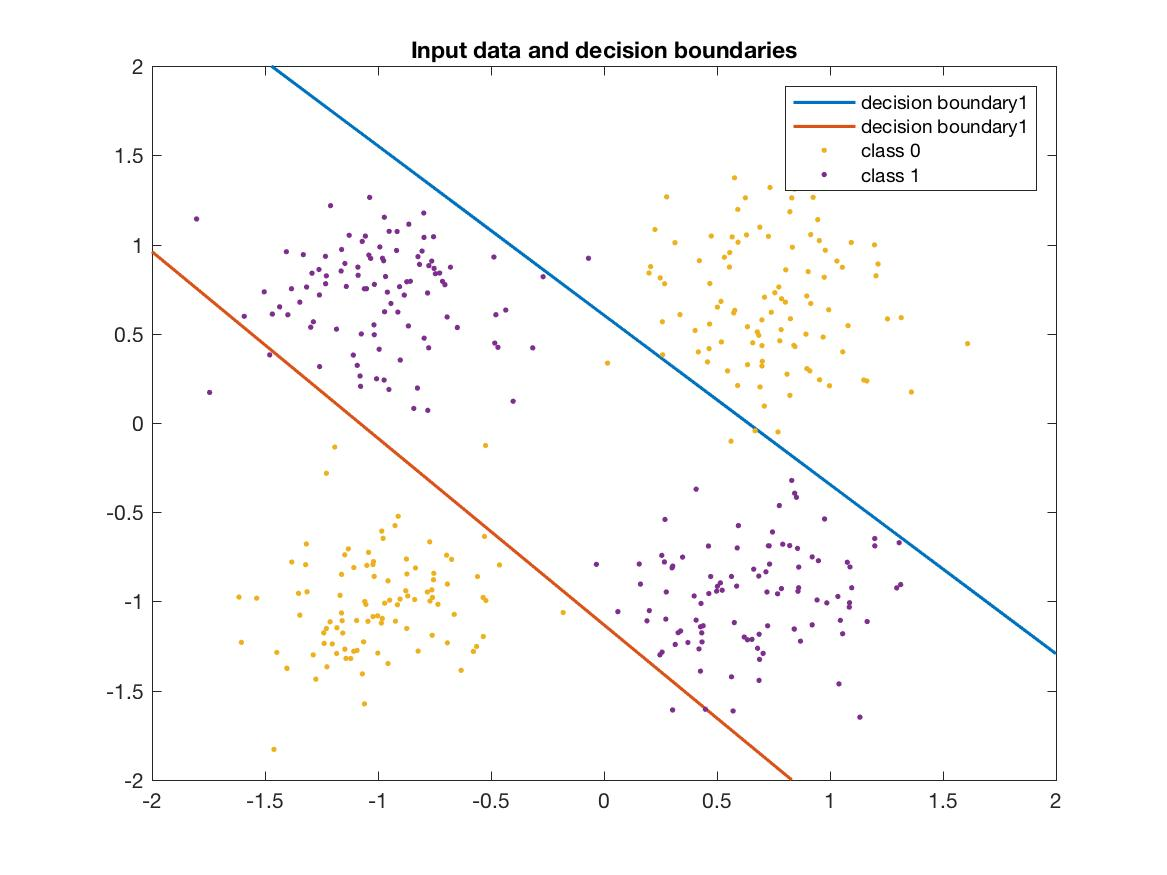
\includegraphics[width = 3.5in]{inputDB.jpg}
\caption{Decision boundaries after networks training with the input data}
\label{inputDB}
\end{figure}

The weight track and final error are also shown below:
\begin{figure}[H]
\centering
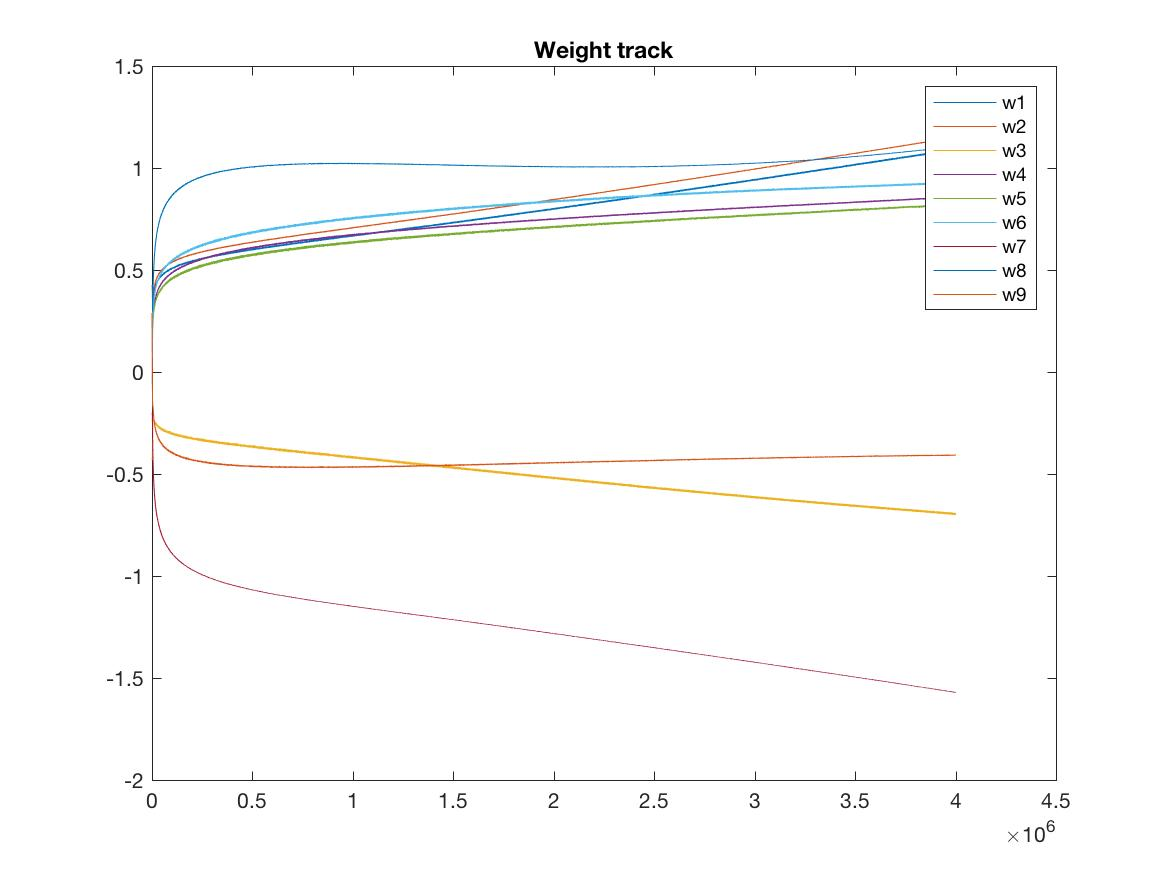
\includegraphics[width = 3.5in]{WT.jpg}
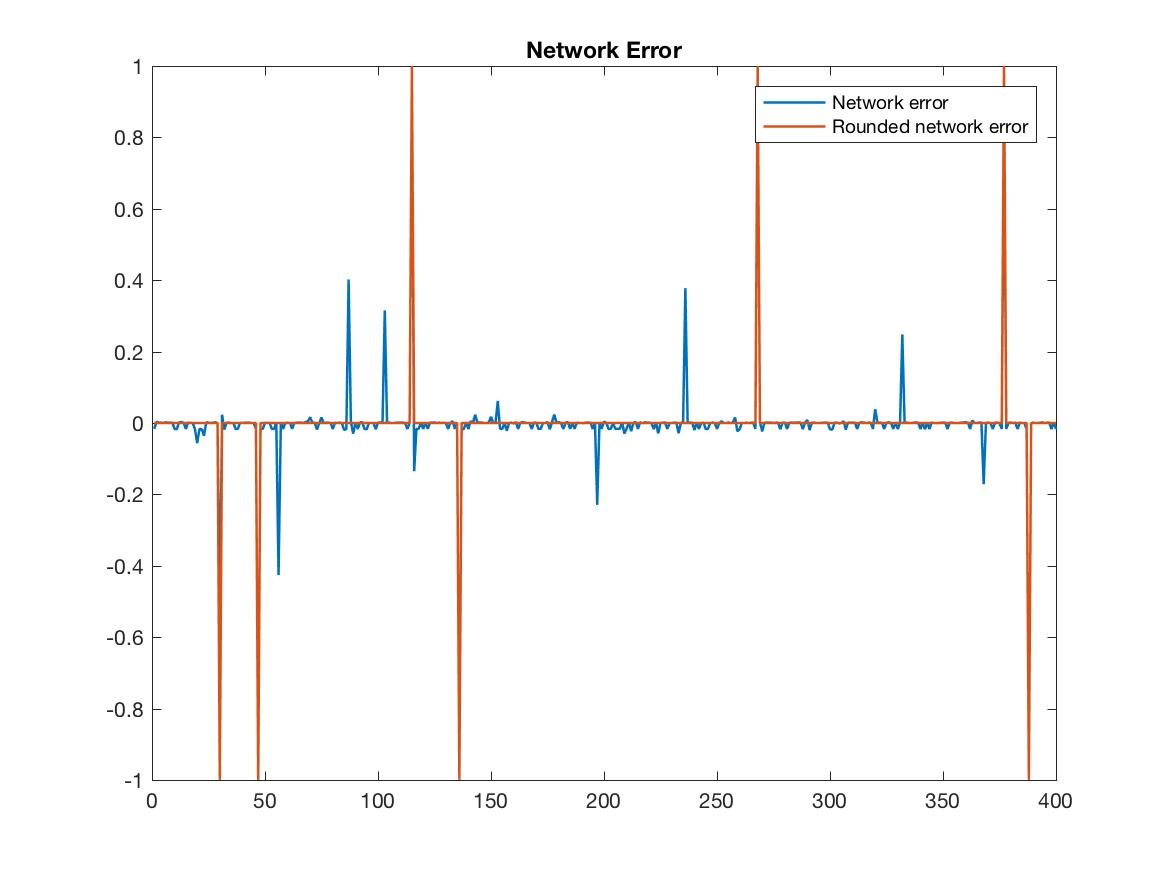
\includegraphics[width = 3.5in]{error.jpg}
\caption{Left: The weight track of the training of the neural network. Right: The resulting error on training data with the trained network.}
\label{WTerror}
\end{figure}

In this case, the number of misclassified points when test on training data is 7. The trained weight values are
$\mathbf{w_1 = 1.0909}$, $\mathbf{w_2 = 1.1500}$, $\mathbf{w_3 = -0.6948}$, $\mathbf{w_4 = 0.8571}$, $\mathbf{w_5 = 0.8169}$, $\mathbf{w_6 = 0.9273}$, $\mathbf{w_7 = -1.5711}$, $\mathbf{w_8 = 1.1047}$, $\mathbf{w_9 = -0.4078}$.\\
The corresponding slope and bias of the two separating boundaries are $\mathbf{k_1 = -0.9486}$, $\mathbf{b_1 = 0.6042}$, $\mathbf{k_2 = -1.0457}$, $\mathbf{b_2 = -1.1314}$. 
 
By observing the pattern of the input data, I assumed that the data points in every quadrant have a bivariate Gaussian distribution. At the same time, the assumption of the x-coordinate and y-coordinate are uncorrelated is made.  With some calculations on the training data, I got the information below:

\begin{table}[htbp]
\centering
\begin{tabular}{|c|c|c|c|c|}
\hline
\ \ & quadrant 1 & quadrant 2 & quadrant 3 & quadrant 4\\
\hline
$\mu_x $ & 0.7309 & -0.9842 & -0.9927 & 0.6551\\
\hline
$\mu_y $ & 0.6684 & 0.7150 & -1.1056 & -0.9730\\
\hline
$\sigma_x^2 $ & 0.0821 & 0.0924 & 0.0761 & 0.0953\\
\hline
$\sigma_y^2 $ & 0.1183 & 0.0771 & 0.0775& 0.0791\\
\hline
\end{tabular}
\end{table}

To generate additional samples that follow the same pattern, I assume the centroids of the data are at $(0.7, 0.7)$, $(-1.0, 0.7)$, $(-1, -1)$, $(0.7, -1)$ for every quadrant respectively. And I assume that the variances of samples in every quadrant is 0.1, and the covariances are 0. I generated 200 samples for each quadrant. The test result is shown below:
\begin{figure}[H]
\centering
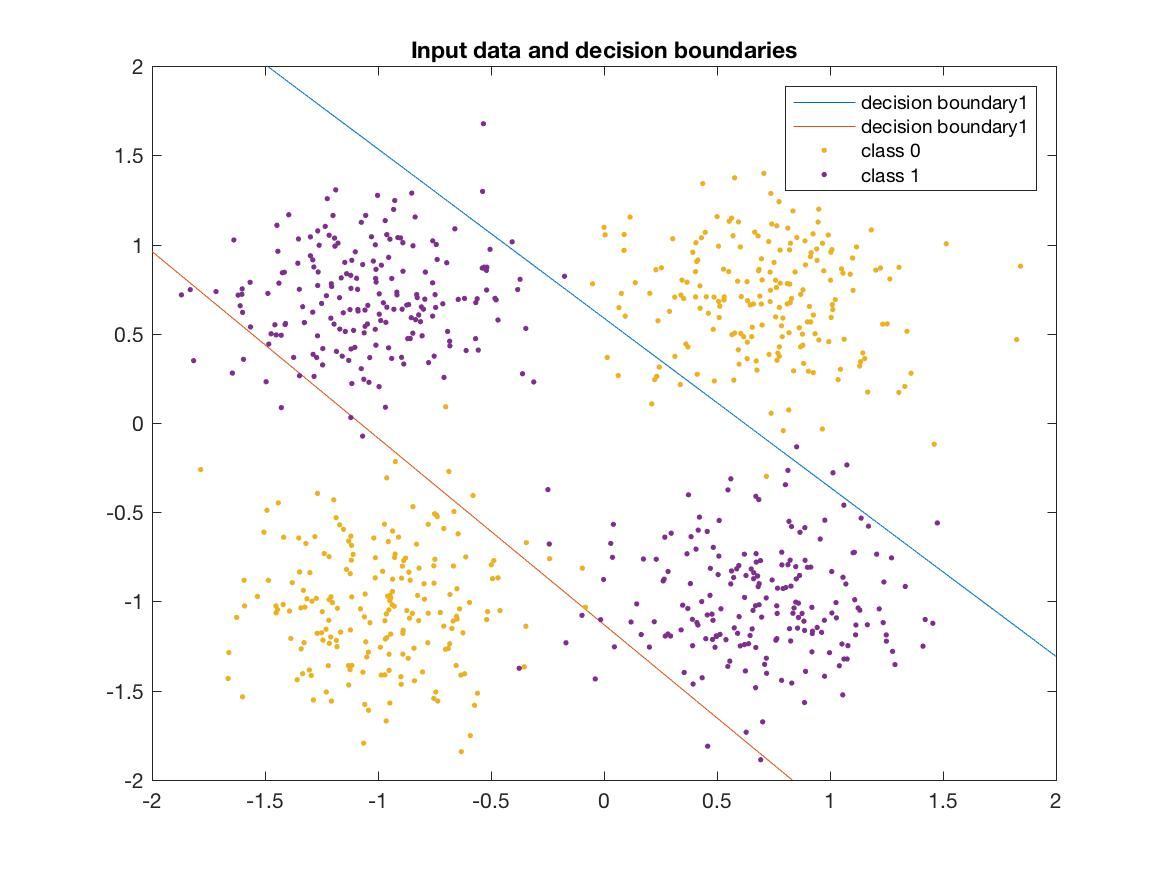
\includegraphics[width = 4.5in]{inputDBtest.jpg}
\caption{Generated data and decision boundaries}
\label{inputDB_test}
\end{figure}

The total number of generated samples is 800. Among these 800 samples, the number of misclassified samples is 27. If I increase the value of the variances, the number of misclassified samples will increase.

Also, if I change the value of $\alpha$ in the sigmoid function, the learned weight values will change:
\begin{table}[htbp]
\centering
\begin{tabular}{|c|c|c|c|c|c|c|c|c|c|}
\hline
$\alpha$ & $w_1$ &$w_2$ & $w_3$ & $w_4$ &$w_5$ & $w_6$ & $w_7$ &$w_8$ & $w_9$\\
\hline
1 & $-3.4560$ & $-3.5102$ & $1.9712$ & $3.9545$ & $3.7752$ & $4.4885$ & $4.5043$ &$4.4643$ & $-6.4618$\\ 
\hline
5 & $-1.4117$ &$-1.4931$ & $0.8701$ & $1.4289$ &$1.3427$ & $1.6087$ & $2.0488$ &$1.9086$ & $-2.9533$\\
\hline
10 & $1.0909$ & $1.1500$ & $-0.6948$ & $0.8571$ & $0.8169$ & $0.9273$ & $-1.5711$ & $1.1047$ & $-0.4078$\\
\hline
\end{tabular}
\end{table}
But the decision boundaries will not vary too much (the corresponding slopes and biases), as shown in the figure below:
\begin{figure}[H]
\centering
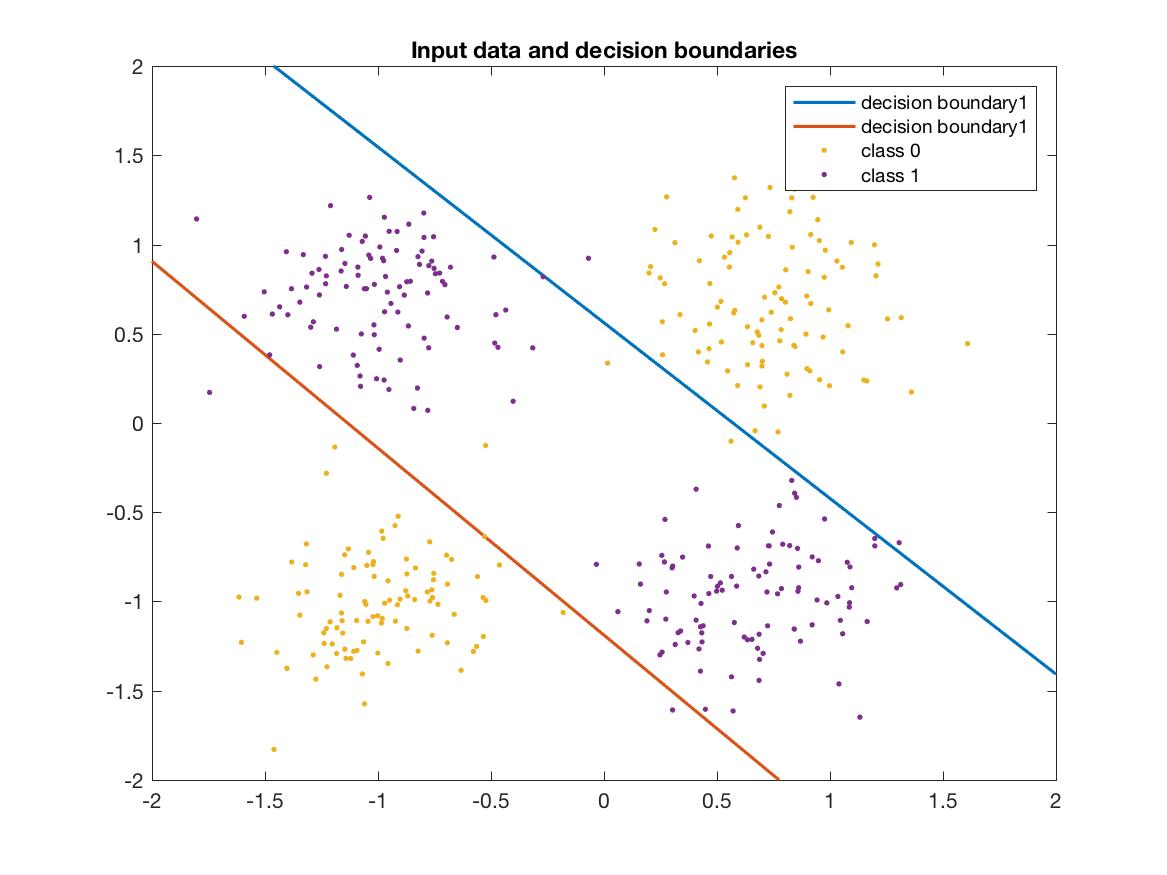
\includegraphics[width = 3in]{inputDB1.jpg}
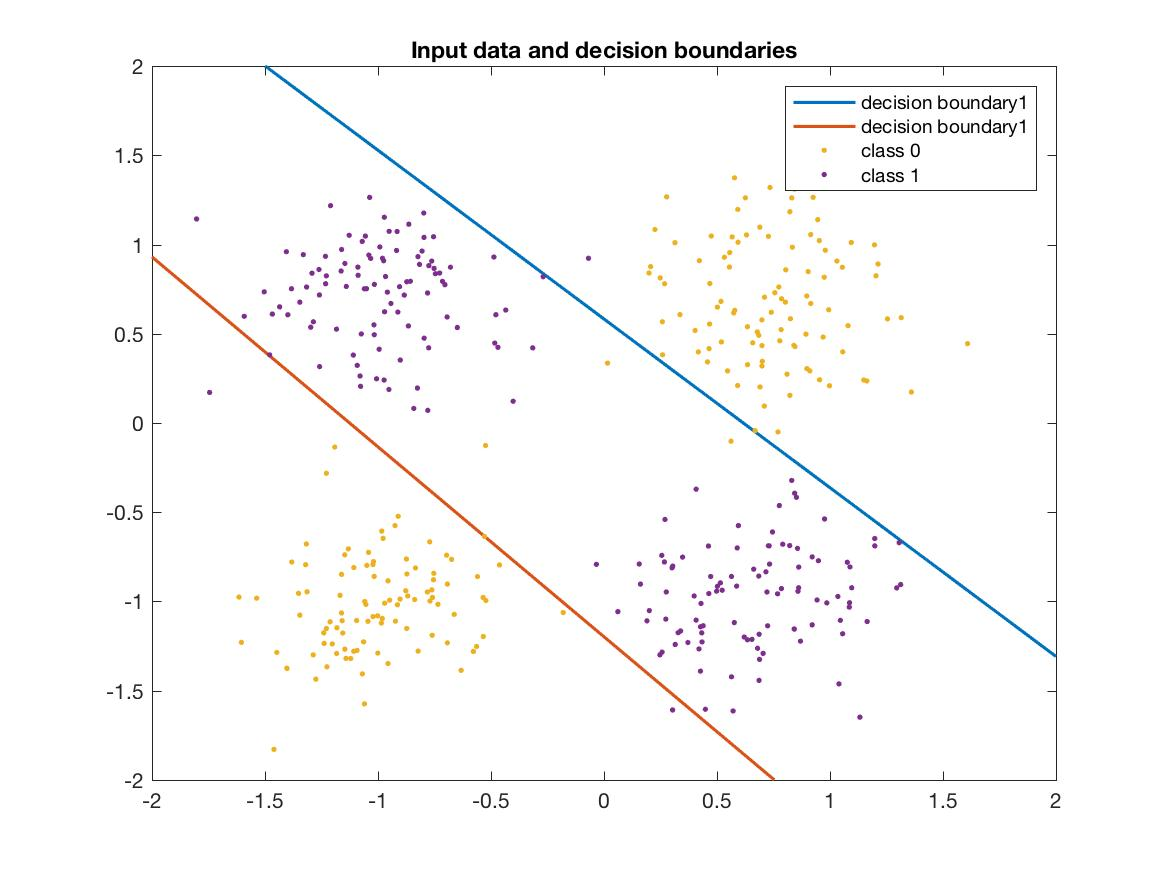
\includegraphics[width = 3in]{inputDB5.jpg}
\caption{Left: Training data and decision boundaries with $\alpha = 1$. Right: Training data and decision boundaries with $\alpha = 5$.}
\label{inputDB_test16nearest}
\end{figure}

\item To solve the same problem, we can have alternative architectures. We can have a hidden layer with 4 elements. As is known to us, the number of elements in the hidden decides the number of lines would be drawn. Instead of drawing only 2 lines, we can also draw 4 separating lines. And then the output from the hidden layer would be either 0 or 1 (assuming using sigmoid activation function), with $2^4$ combinations of either 0 or 1 output . Then the output of the hidden layer would be merged into decision of either 0 or 1(2 classes) assuming either all 1 or all 0 output from 4 elements of the hidden layer to be class 0, others to be class 1, by adjusting the weight coefficients for the output layer.

We can also have more than 4 processing elements in the hidden layer by the same concept. The more elements, the accurate the classification result, assuming we have enough data.

What is more, we can have more than one hidden layers. Every element in the 1st hidden layer define a line, we will have $2^n$ lines assuming we have n processing elements in the 1st hidden layer. For every coming hidden layer, we merge the result from the 1st hidden one at a time.

In this problem, I would choose the model I mentioned at the beginning of this report. Because this model is the simplest model. And if we use a complicated model, the performance of the model may be better, but since we have already trained a model which works for this problem, we should choose a simpler model. 
What is more, as inspired by the curse of dimensionality, the more complex the model, the more coefficients we will have to train, the more training data we need. Given the data we have, the complexity of the model I mentioned at the beginning of this report is enough.

\item I chose the total 16 points from nearest to the origin, as well as farthest to the origin. The results are shown below with no classification error on training data:

\begin{figure}[H]
\centering
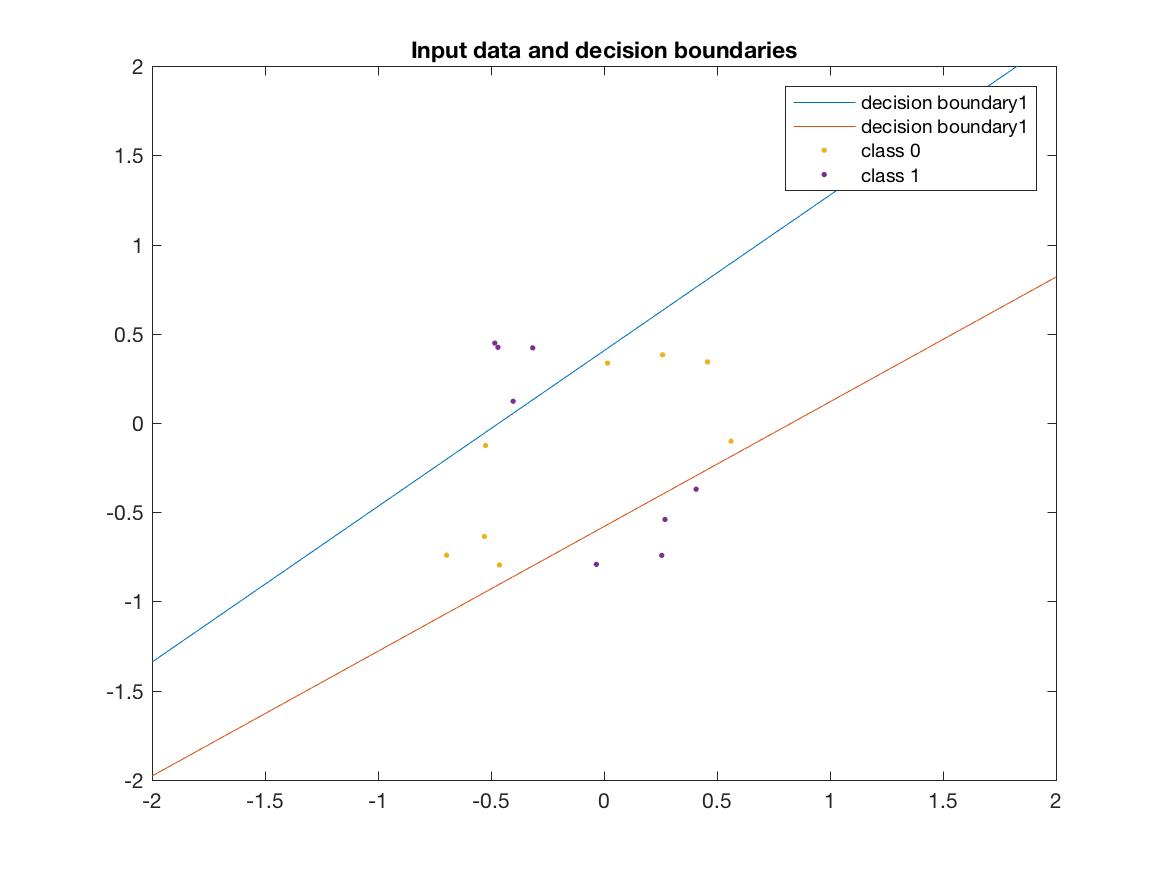
\includegraphics[width = 3.5in]{inputDBonly16nearest.jpg}
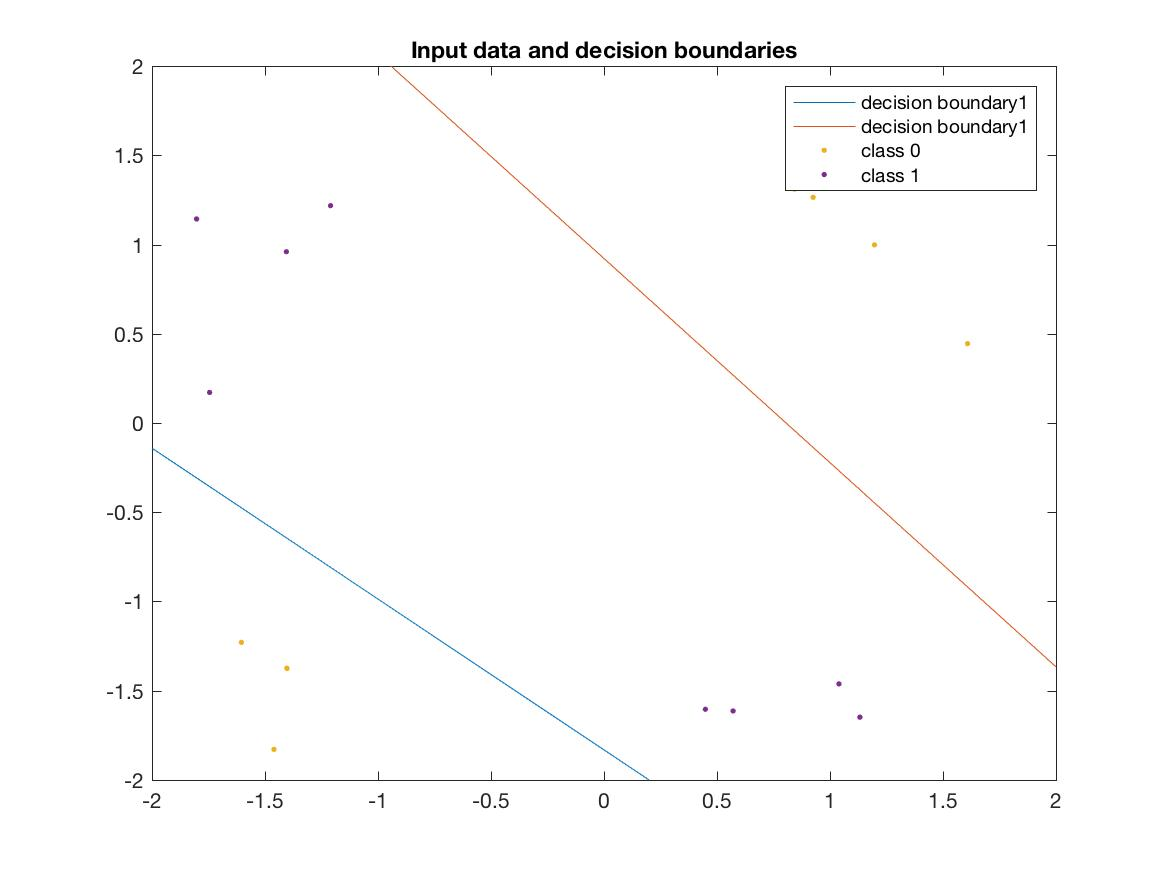
\includegraphics[width = 3.5in]{inputDBonly16farthest.jpg}
\caption{Left: 16 data nearest to the origin and decision boundaries. Right: 16 data farthest to the origin and decision boundaries}
\label{inputDB_test16nearest}
\end{figure}

The corresponding weight values when the samples are chosen to be nearest to the origin, are $\mathbf{w_1 = -0.8320}$, $\mathbf{w_2 = 0.9515}$, $\mathbf{w_3 = -0.3849}$, $\mathbf{w_4 = -0.8232}$, $\mathbf{w_5 = 1.1833}$, $\mathbf{w_6 = 0.6463}$, $\mathbf{w_7 = 1.3517}$, $\mathbf{w_8 = -1.1856}$, $\mathbf{w_9 = 0.5027}$.

The corresponding weight values when the samples are chosen to be farthest to the origin, are $\mathbf{w_1 = -0.2697}$, $\mathbf{w_2 = -0.3166}$, $\mathbf{w_3 = -0.6063}$, $\mathbf{w_4 = 0.4827}$, $\mathbf{w_5 = 0.4212}$, $\mathbf{w_6 = -0.5102}$, $\mathbf{w_7 = -0.8288}$, $\mathbf{w_8 = -0.7747}$, $\mathbf{w_9 = 0.4003}$.

As can be seen, though the decision boundaries are able to separate the training data totally, but it is obvious that neither of these two sets of decision boundaries are the best solution. Which is obvious that it is hard for us to generate a model with too less the number of samples - these number of samples is not enough to represent the pattern of the whole data set.

The best solution would be the model trained by using much data, as shown before, using all the data. 

Sixteen points are too far from enough to represent the pattern of the whole data set, thus the situation shown above would occur - different solution for the same problem - the decision boundaries have totally different slopes.

\item If I were to choose hand-select the parameters of the network, there are two simplest model come to mind, the structures as well as the decision boundaries are shown below in figures \ref{models} and \ref{modelsplot}.
\begin{figure}[H]
\centering
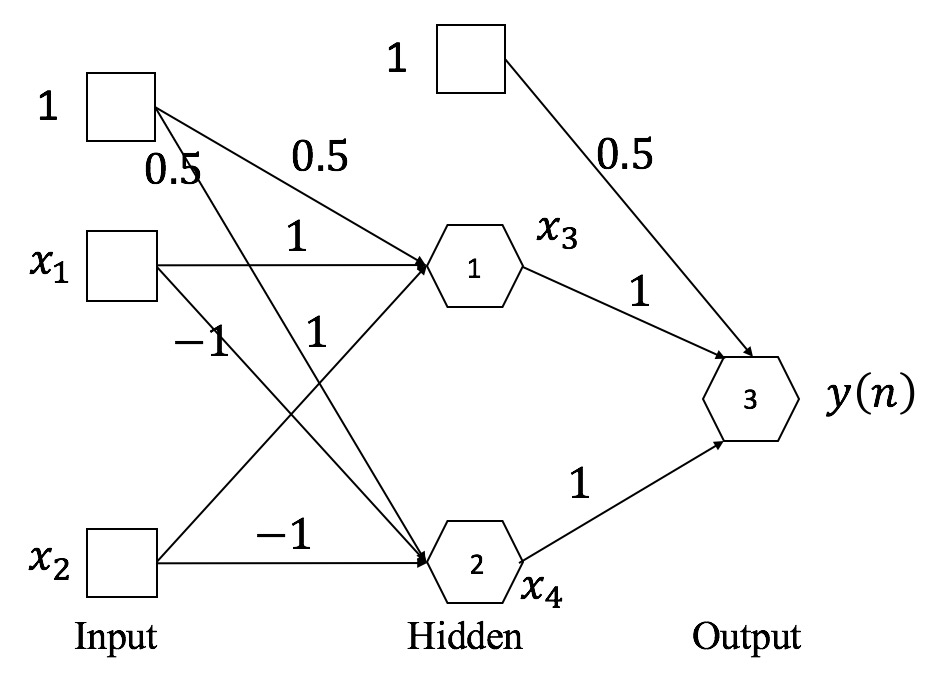
\includegraphics[width = 3.5in]{positive.jpg}
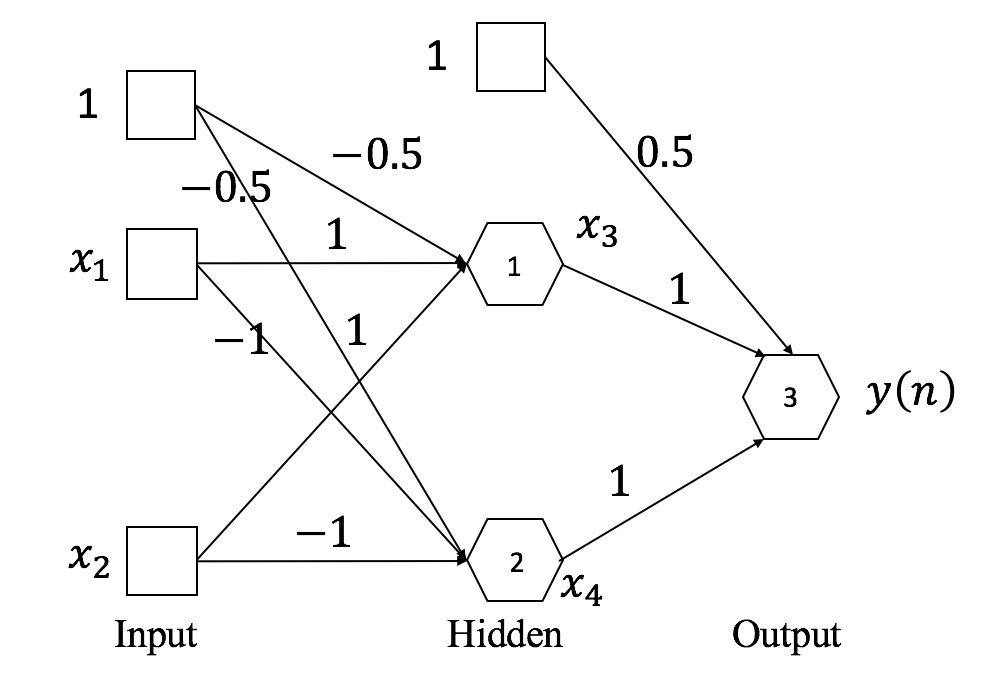
\includegraphics[width = 3.5in]{negative.jpg}
\caption{Two way of building models theoretically}
\label{models}
\end{figure}

\begin{figure}[H]
\centering
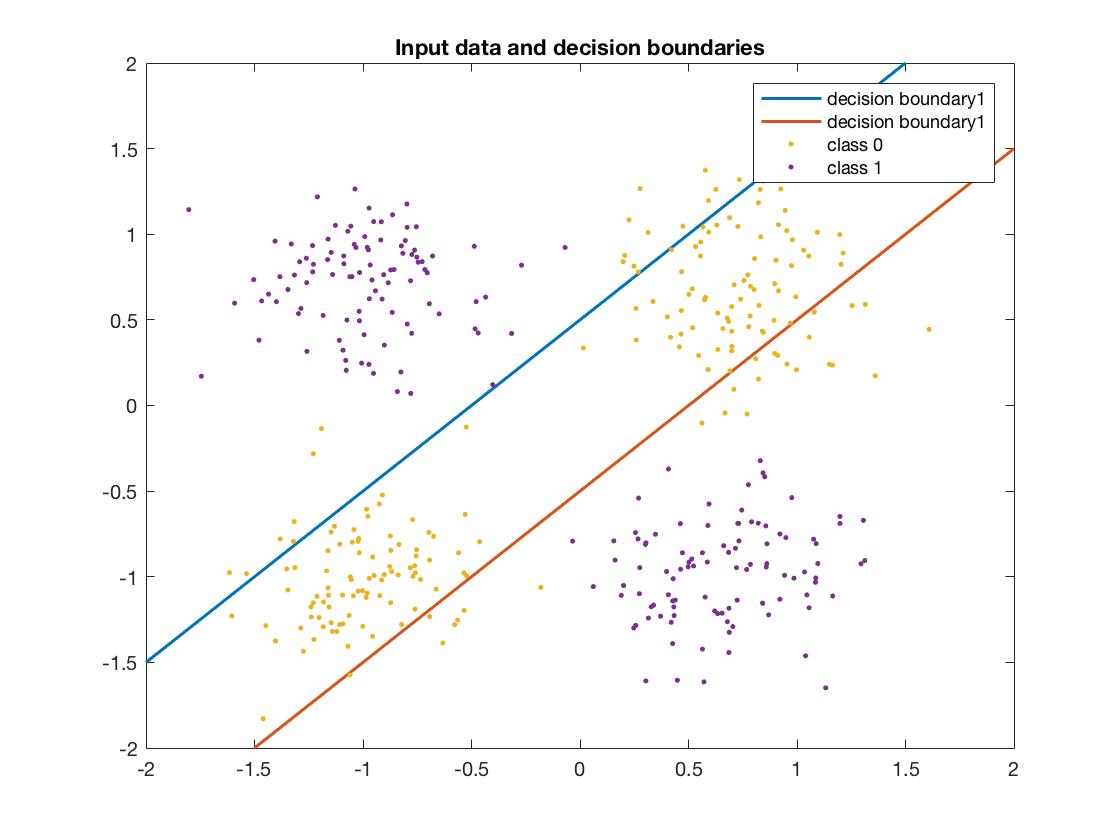
\includegraphics[width = 3.5in]{positiveplot.jpg}
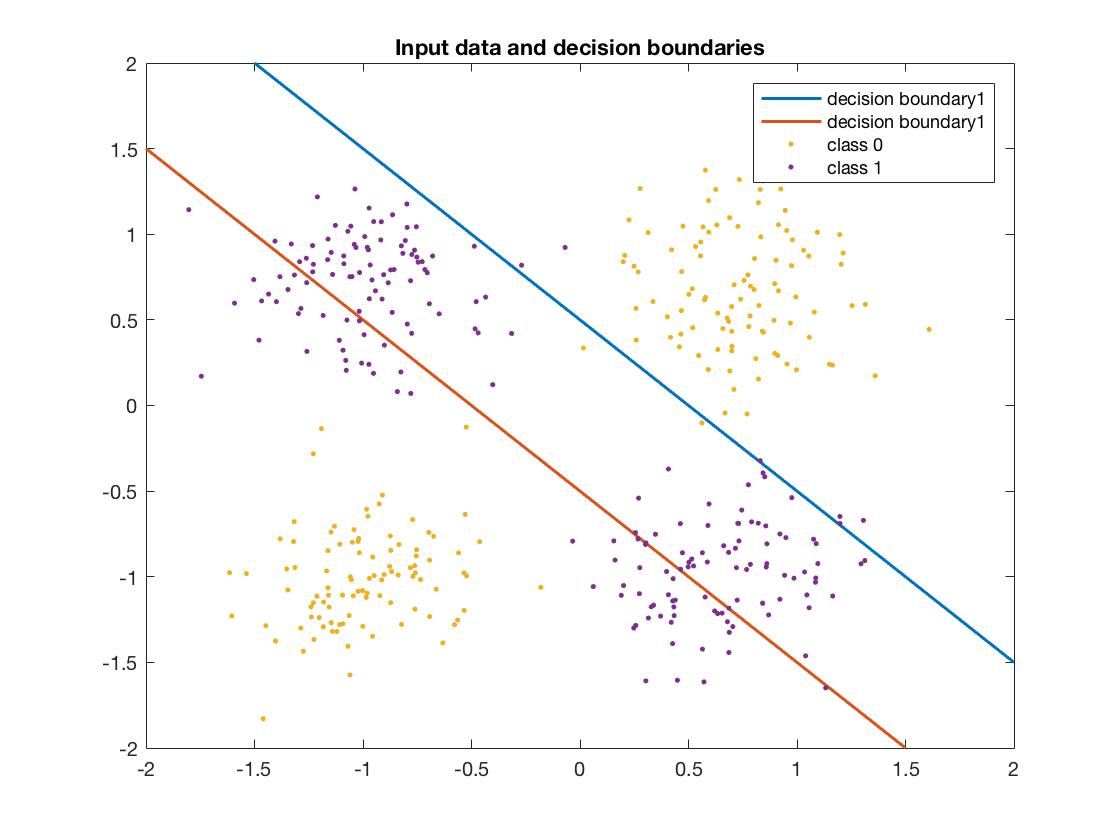
\includegraphics[width = 3.5in]{negativeplot.jpg}
\caption{Corresponding decision boundaries with samples of this problem.}
\label{modelsplot}
\end{figure}

Those shown above are only theoretical models - the decision boundaries are two parallel lines, with either positive slopes or negative slopes.

 Based on the given samples, I would choose the weight values such that the slope of the 1st line $k_1 = -\displaystyle\frac{w_1}{w_2} \approx -0.9$, the bias of the 1st line $b1 = -\displaystyle\frac{w_3}{w_2} \approx 0.6$, the slope of the 2nd line $k_2 = -\displaystyle\frac{w_4}{w_5} \approx -1.0$, the bias of the second line $b2 = -\displaystyle\frac{w_6}{w_5} \approx -1.1$. These values only gives the range of the ratios(relationships) of corresponding weights. And I would choose $w_7 = -1$, $w_8 = 1$, $w_9 = -0.5$. I would say that based on the samples given, the optimal decision boundaries may not be parallel. 

And as mentioned before, the magnitude of each weight has something to do with the value of $\alpha$ in the activation function, but it will not affect the decision boundary. So I would simply choose the magnitude of weights to be near 1, i.e. $w_1 = 0.9$, $w_2 = 1$, $w_3 = -0.6$, $w_4 = 1$, $w_5 = 1$, $w_6 = 1.1$, $w_7 = -1$, $w_8 = 1$, $w_9 = -0.5$.

\begin{figure}[H]
\centering
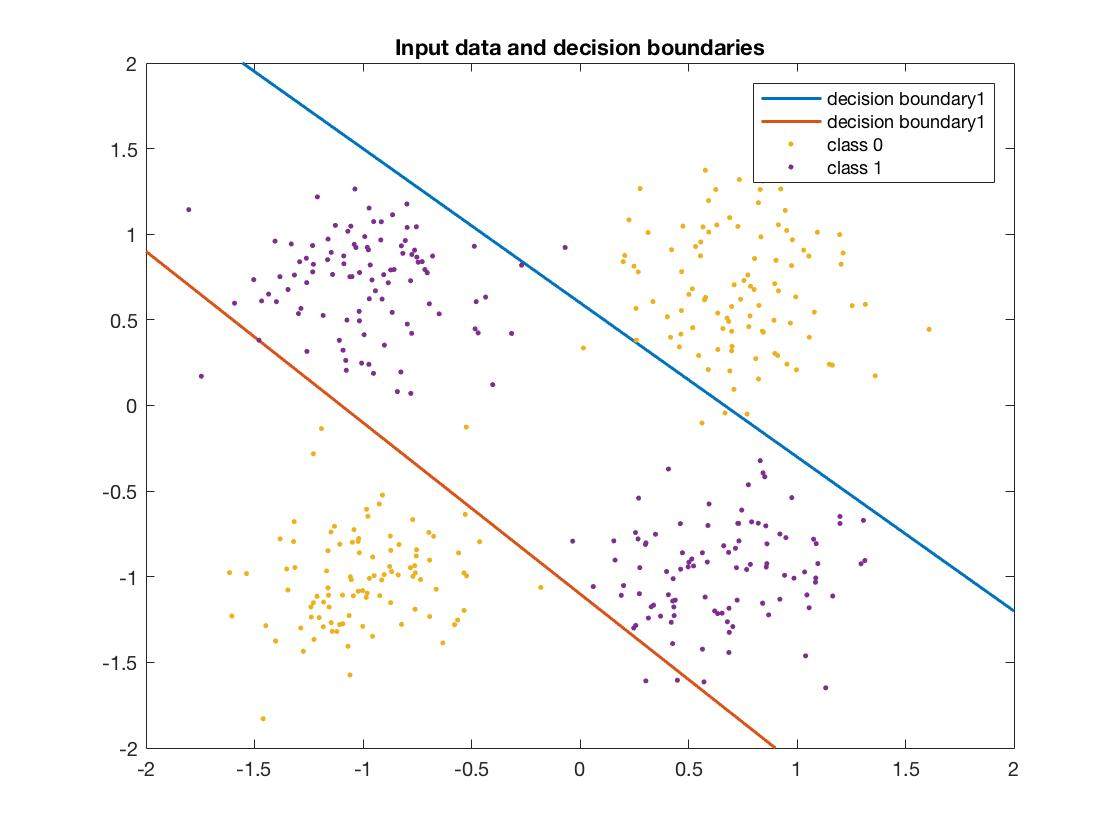
\includegraphics[width = 3.5in]{theoretical.jpg}
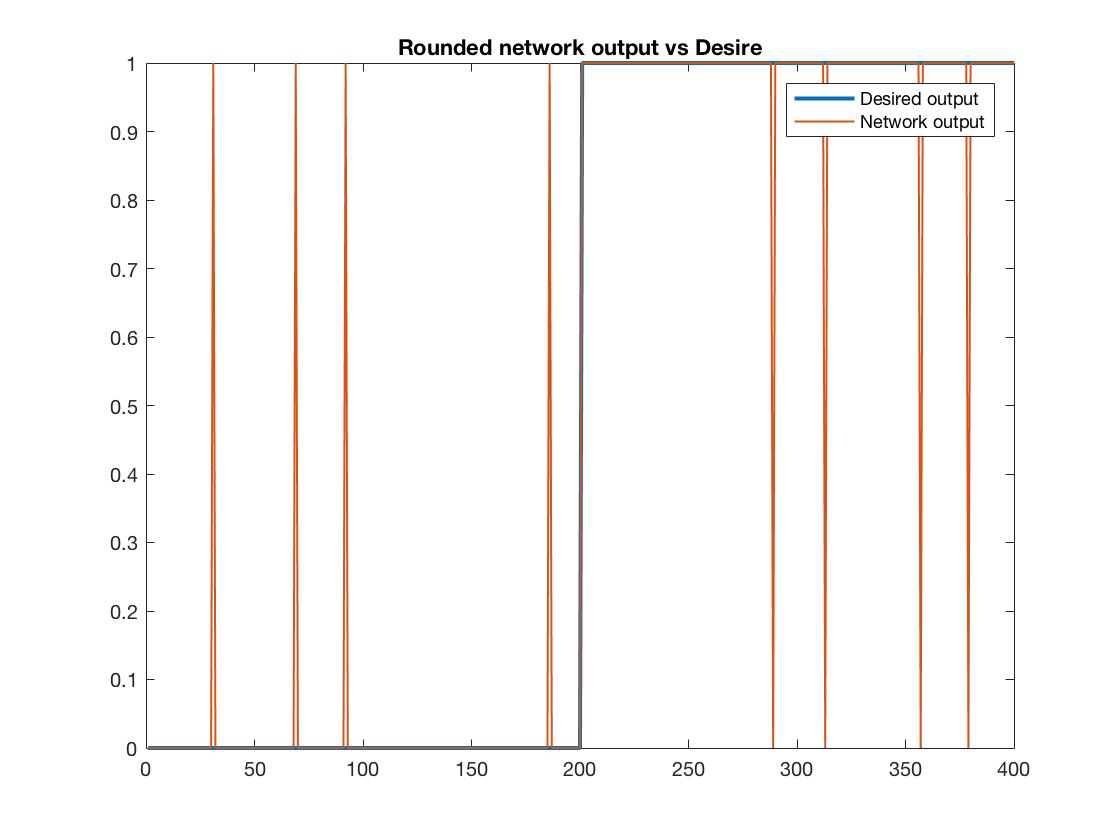
\includegraphics[width = 3.5in]{theoerror.jpg}
\caption{Left: Decision boundary of the network with hand-selected parameters. Right: Eight errors occur with the net work using hand-selected parameters.} 
\label{modelsplot}
\end{figure}

And also, the multi-layer neural network learned the solution as I expected, except for the magnitude differs with different $\alpha$ used in the sigmoid function. I got the lines with either positive slopes or negatives. Either models give similar performance.

\item There are several methods to improve the generalization accuracy of the multi-layer neural network:
\begin{enumerate}
\item If possible, collect more data to train the network. As is known, more training data would let the distribution be much more clear and hence improve accuracy.

\item Randomize the data before model training. The data we got is aligned in a good order, i.e. the labels for the first 200 samples are all 0, and the labels for the last 200 samples are all 1. This order would cause the error (i.e. $e(n) = d(n)-y(n)$) has a big change every time the procedure changes from 200th sample to 201st sample, which we would see a big change of weight at that point, thus it is possible to lead us the weight near a local optimal. And later on we would stuck at local minimum. Randomization can avoid this problem of suddenly step into a region near local optimal.

\item Use mini batch instead of online learning. Since the weight update as average value, it can avoid the problem of stuck at local optimal.

\item We can choose other activation functions such as the hyperbolic tangent function. Since the sigmoid function actually changes the error space. 

\item We can also add a momentum term multiplying by a parameter to the update equation, i.e.\\
\begin{center} $w_j(n+1) = \eta \delta_j(n)y_j(n) + \lambda \Delta w_j(n-1)$ \end{center}

\item For the initialization of the weight values, we should avoid all zeros. And most importantly, we should avoid the value of $\sum_{i}w_ix_i+b$ being out of the ``active" range of the activation function. As shown in the figure below, when the values of alpha is different, the range that the gradient of the activation function actually changes (``active range") is different. We should choose some initial values of weight based on our data to avoid starting at some point that the gradient of activation function is not changing at all, thus the weight will not update at all.

\begin{figure}[H]
\centering
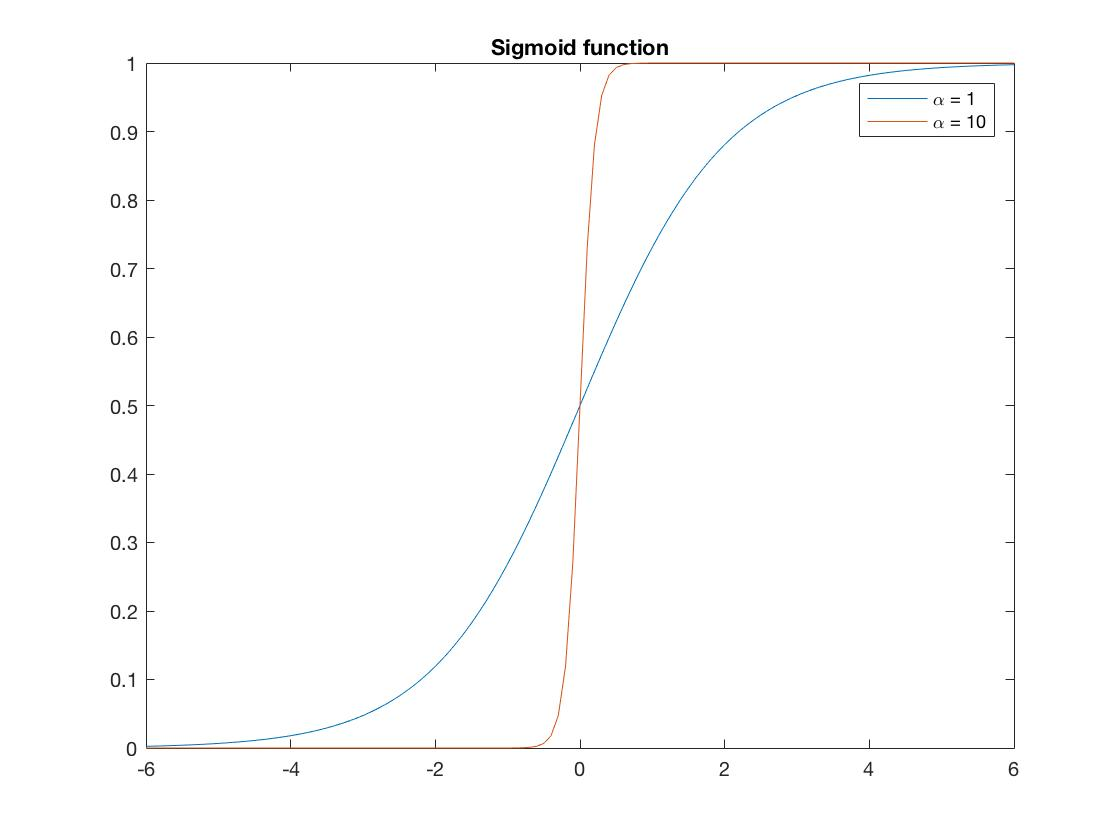
\includegraphics[width = 4.5in]{sigmoid.jpg}
\caption{The sigmoid function with different values of $\alpha$}
\label{sigmoid}
\end{figure}

\item Using cross validation to choose a best model.

\end{enumerate}

\end{itemize}

\newpage
\Large{The MATLAB code used in this report:}\\
\normalsize
\large{Main script:}
\normalsize
\begin{lstlisting}
clear
close all
clc
dbstop if error
data = importdata('HW6_Data.txt');
%% 
num_iter = 10000;
% randomization
traindata = data;
% traindata = [data_sorted{1,1}(end-3:end, :); data_sorted{1,2}(end-3:end, :); data_sorted{1,3}(end-3:end, :); data_sorted{1,4}(end-3:end, :)]; 
num_data = size(traindata,1);
for ii = 1:num_iter
    r(:,1+num_data*(ii-1):1+num_data*(ii-1)+num_data-1) = randperm( num_data ); 
    data_re = traindata(r(:,1+num_data*(ii-1):1+num_data*(ii-1)+num_data-1),:);
    x(1+num_data*(ii-1):1+num_data*(ii-1)+num_data-1,:) = data_re(:,1:2);
    d(1+num_data*(ii-1):1+num_data*(ii-1)+num_data-1,:) = data_re(:,3);
end
x(:,3) = ones(size(x,1),1);
alpha = 5;
eta = 0.001;
w = random('unif', -1/sqrt(2), 1/sqrt(2), length(d), 9); % initialize 
a = 0;

tic
[ ~, w, error] = back_prop( x, d, w, alpha, eta, 1);
weight = w(end,:);
[y, ~] = back_prop( x(1:num_data,:), d(1:num_data, :), w(end,:),alpha, eta, 1);
toc

desire = d(1:num_data, :);
output = round(y(end-num_data+1:end, :));
r0 = find(desire == 0);
de = desire(r0,:);
op = output(r0,:);
r1 = find(desire == 1);
de = [de; desire(r1,:)];
op = [op; output(r1,:)];
figure, plot(de, 'Linewidth', 2), hold on
plot(op, 'Linewidth', 1),title('Rounded network output vs Desire')
legend('Desired output', 'Network output')
saveas(gcf,['DvsYrounded' num2str(alpha) '.jpg']);

figure, plot(d(1:num_data, :)-y(end-num_data+1:end, :), 'Linewidth', 1.2), title('Network Error')
hold on, plot(d(1:num_data, :)-round(y(end-num_data+1:end, :)), 'Linewidth', 1.2)
legend('Network error', 'Rounded network error')
saveas(gcf,['error' num2str(alpha) '.jpg']);

figure, plot(w), title('Weight track'), legend('w1', 'w2', 'w3', 'w4', 'w5', 'w6', 'w7', 'w8', 'w9')
saveas(gcf,['WT' num2str(alpha) '.jpg']);

xx1 = -2:0.1:2;
yy1 = -weight(:,1)*xx1/weight(:,2)-weight(:,3)/weight(:,2);
yy2 = -weight(:,4)*xx1/weight(:,5)-weight(:,6)/weight(:,5);
figure
plot(xx1, yy1, 'Linewidth', 1.5), hold on, plot(xx1, yy2, 'Linewidth', 1.5), hold on
inputx1 = x(1:num_data,1);
inputx2 = x(1:num_data,2);
plot(inputx1(d(1:num_data) == 0), inputx2(d(1:num_data) == 0),'.', 'Linewidth', 10), hold on
plot(inputx1(d(1:num_data) == 1), inputx2(d(1:num_data) == 1),'.', 'Linewidth', 10)
axis([-2 2 -2 2]);
title('Input data and decision boundaries')
legend('decision boundary1','decision boundary1', 'class 0', 'class 1')
saveas(gcf,['inputDB' num2str(alpha) '.jpg']);

num_wrong = sum(abs(round(y)-d(1:num_data)));
display(['Number of misclassified points is ' num2str(num_wrong)])

weight = w(end,:);
save(['weight' num2str(alpha) '.mat'],'weight')
\end{lstlisting}

\large{Function}
\normalsize
\begin{lstlisting}
function [ y, w, error ] = back_prop( x, d, w, alpha, eta, type_activeF)
% function [ y, w, b, x3, x4 ] = back_propagation( x, d, w, b, alpha, eta)
%function of back propagation
%   x: input data
%   x: desired output values
%   w: old weight
%   alpha: alpha value for the activation function (sigmoid or tanh)
%   eta: step size
%   type_activeF: 1 for sigmoid (logistic), 2 for tanh

for n = 1:length(d)
    
    %% Forward pass
    % 1st layer
    x1(n,:) = x(n,1);
    x2(n,:) = x(n,2);
    
    net1(n,:) = x(n,:)*w(n,1:3)';
    [ x3(n,:), deriva_x3 ] = activation( net1(n,:), alpha, type_activeF);

    net2(n,:) = x(n,:)*w(n,4:6)';
    [ x4(n,:), deriva_x4 ] = activation( net2(n,:), alpha, type_activeF);
    
    % 2nd layer(hidden)
    net3(n,:) = [x3(n,:) x4(n,:) 1]*w(n,7:9)';
    [ y(n,:), deriva_y ] = activation( net3(n,:), alpha, type_activeF);
    
    %% Backward pass
    % 2nd layer(hidden)
%     delta_w(1,:) = w(1,:);
    error(n,:) = abs(d(n,:)-y(n,:));
    delta3(n,:) = (d(n,:) - y(n,:))*deriva_y;
    w(n+1,7:9)  = w(n,7:9) + eta * delta3(n,:)*[x3(n,:) x4(n,:) 1];
%     w(n+1,7:9)  = w(n,7:9) + eta * delta3(n,:)*[x3(n,:) x4(n,:) 1] + a*delta_w(n,7:9); % update the weight values for net 3 (w7, w8, w9)

    % 1st layer
    delta1(n,:) = deriva_x3*delta3(n,:) * w(n,7);
    w(n+1,1:3)  = w(n,1:3) + eta * delta1(n,:)*x(n,:);
% 	w(n+1,1:3)  = w(n,1:3) + eta * delta1(n,:)*x(n,:) + a*delta_w(n,1:3); % update the weight values for net 1 (w1, w2, w3)
    
    % 2nd layer
    delta2(n,:) = deriva_x4*delta3(n,:) * w(n,8);
    w(n+1,4:6)  = w(n,4:6) + eta * delta2(n,:)*x(n,:);
%     w(n+1,4:6)  = w(n,4:6) + eta * delta2(n,:)*x(n,:) + a*delta_w(n,4:6); % update the weight values for net 3 (w7, w8, w9)
    
% 	delta_w(n+1,:) = w(n+1,:)-w(n,:);
end
end

function [ output, derivative ] = activation( input, alpha, type_activeF)
    if type_activeF == 1
        output = logistic( input, alpha );
        derivative = alpha*output*(1-output);
    elseif type_activeF == 2
        output = tanh(alpha*input);
        derivative = alpha*(1-output^2);
    end
end

function fx = logistic( x, alpha )
%logistic sigmoid fuction
%   x: input value
%   alpha: parameter in the logistic sigmoid function
    fx = 1./(1+exp(-alpha*x));

end


\end{lstlisting}
\end{spacing}
\end{document}